\documentclass[10pt]{article}
\usepackage[margin=1in]{geometry}
\usepackage[T1]{fontenc}
\usepackage{lmodern}
\usepackage{microtype}
\usepackage{amsmath,amssymb}
\usepackage{booktabs}
\usepackage{array}
\newcolumntype{L}[1]{>{\raggedright\arraybackslash}p{#1}}
\usepackage{graphicx}
\usepackage[numbers,sort&compress]{natbib}
\usepackage{xcolor}
\usepackage{tikz}
\usetikzlibrary{positioning,arrows.meta}
\usepackage[hidelinks]{hyperref}
\usepackage{caption}
\captionsetup{font=small,labelfont=bf}

\newcommand{\Rec}{\mathrm{R}}
\newcommand{\Acc}{\mathrm{Acc}}
\newcommand{\TBD}[1]{\textcolor{red}{[TBD: #1]}}

\title{What a Recipient Can Recover from a Useful Prediction:\\
An Evaluation of Feature Defenses and Output Contracts on Stored Representation Models}
\author{Anonymous authors}
\date{}

\begin{document}
\maketitle

\begin{abstract}
Methods that protect a declared attribute in a learned representation come with checks that cover a particular object
and a particular class of attackers. A recipient served by a multi-purpose model may receive more than that object: a
task output instead of, or together with, protected features, and two recipients that serve the same person may link
what they receive. We ask what a recipient can recover about the attribute from everything it receives, alone or linked
with a second recipient, and how useful the release remains. On stored Adult and HMDA representation models we apply
each method's own check and then attack every released surface with one slate of attackers fitted on labelled releases
of other records. Official LEACE meets its linear bound, yet nonlinear attackers recover the attribute about as well as
from untreated features (AUC 0.817 against 0.815 on Adult and 0.863 against 0.870 on HMDA); the guarantee covers linear
classifiers, so this recovery lies outside its scope. Because the untreated model's task output alone already reveals
the attribute, releasing it beside noisy or FARE features brings recovery back to 0.76--0.79. When each treatment
releases the output of a useful logistic-regression head, FARE lowers sex recovery from that score from 0.773 to 0.539,
but a tree of the same budget without the fairness term accounts for about half of the reduction, and FARE's accuracy is
not shown to stay within one point. In the one coalition we evaluated, two recipients granted perfect linkage recover
more than either alone, even from decisions. All results are exploratory evidence on data used by earlier analyses,
under a declared threat model; we propose no new method and no privacy guarantee.
\end{abstract}

\section{Introduction}

Methods that protect a declared attribute in a learned representation are stated and checked on that representation.
LEACE erases the linearly available information about the attribute: on the distribution it is fitted to, no linear
classifier reading the erased representation does better than a constant predictor under any convex
loss~\citep{belrose2023leace}. FARE maps records to a finite set of cells and certifies, with high probability, a bound
on the demographic-parity distance of any classifier that reads only the cell~\citep{jovanovic2023fare}. The
purpose-specific encoders we study were trained so that a linear probe's $R^2$ for each disallowed attribute stays below
a threshold. Each of these promises is precise about two things, the object it covers and the attackers it covers.
Neither has to match what a recipient of the system receives or how the recipient can analyse it.

A release policy is defined by what each recipient receives. As an illustration, and not a description of any
documented deployment, consider a service that holds records about people and serves two recipients with different
permitted purposes: one receives a prediction of income, the other a prediction of an occupation group, and neither may
use a declared attribute such as sex or race. For each person it serves, a recipient receives the output of its own task
(a score, a probability vector or a decision) and possibly the features that produced it. The policy is written per
recipient, but the person is shared. A recipient may know whom an output describes, so two recipients that serve the
same person could link their outputs by record, and a recipient that knows the protected attribute for some of the
people it serves could learn how outputs relate to that attribute. Under these conditions a defense applied to the
features addresses only part of what recipients see: the task output may carry what was removed from the features, a
recipient may hold features and output together, and two recipients may pool linked outputs. We know of no source that
documents a deployment with all of these properties, so we do not claim that one exists.

These conditions raise a narrow question, which this paper studies. For stored representation models and published
defenses, what can a recipient recover about a declared protected attribute from everything it receives, alone or
linked with one other recipient, and how useful is that release for the recipient's task? We answer it under a declared
threat model (Section~\ref{sec:threat}). The recipient holds exactly its release, the attacker learns from a labelled
sample of other records' releases from the same population, and a pair of recipients is granted perfect linkage. Other
access, such as a recipient that also holds a person's inputs, public model parameters or permission to query
repeatedly, defines a different threat model, which we do not test and do not dismiss.

We study six stored purpose-specific encoders trained on Adult and HMDA. For each, we first apply each method's own
protection check and then measure recovery from the surfaces a recipient receives under the evaluated contracts: the
representation; the task output in four formats (full logits, centred logits, probabilities and hard decisions);
features and output together; and the outputs of two recipients linked by record. The same slate of linear, tree and
neural attackers, fitted and selected on held-out roles, attacks every surface. Recovery is read beside held-out
utility, which in the later experiments is the utility of the head whose output is released and in the earlier ones
that of a refitted probe (Section~\ref{sec:protocol}). A tree of the same budget as FARE's but without its fairness term
separates the effect of that term from the effect of compression.

The results separate three situations that a single recovery figure would conflate. A method can pass its own check
while recovery continues outside the check's scope: official LEACE meets its linear bound on every map, and nonlinear
attackers recover the attribute about as well as from untreated features. The encoders' own constraint is a different
case, because their stored linear check fails on 11 of 42 combinations of purpose--attribute pair and encoder seed.
Recovery can also come through a surface that a feature defense does not cover: output-only recovery exceeds that of a
label-only reference, so a defense applied to the features cannot be credited with protection when the original output
accompanies them. Low recovery has to be read together with utility. The frozen task heads' hard decisions leak little,
but they barely beat a constant. When every treatment releases a useful head, FARE's score recovers much less than the
untreated or LEACE score, yet about half of that reduction is reproduced by a same-budget tree without the fairness
term, and on an easier task the tree reproduces most of it. In the one coalition we evaluated, two recipients with
perfectly linked outputs recover more than either alone, even when each receives only decisions.

None of this shows that LEACE or FARE fails its own promise: LEACE's held wherever we could check it, and FARE's
certificate was too weak at our certification sizes to be checked. The encoders' stored check is the exception. What
the results show is what a method must address if it aims to limit what recipients can learn: the complete release
under a stated access model, the utility of the output that is actually released, a capacity-matched control for any
effect claimed for a fairness term, and the linked view of recipients that serve the same people
(Section~\ref{sec:discussion}). The individual observations, that linear protection does not stop nonlinear recovery,
that outputs leak beyond labels, that hard labels are not a defense in general and that combined releases can leak
more, are known (Section~\ref{sec:related}). This paper measures them together, with utility, on the same models and
under one stated threat model, and adds two quantities specific to these models: the share of FARE's effect that a
capacity-matched tree reproduces, which differs between settings, and the gap in recovery between useful scores and
equally accurate decisions. Every assessment row had been used by earlier analyses of these models, so the results are
exploratory development evidence rather than fresh confirmation, and intervals are conditional on the fitted heads and
attackers. We propose no new algorithm, no population privacy guarantee and no composition theorem.

\section{Setting}\label{sec:setting}

\paragraph{Data.} Adult is the UCI census-income data; HMDA is the 2023 California loan-application register (home
purchase, first lien, site-built). Each dataset has three purposes, each with a task and a list of disallowed attributes.
On Adult these are income prediction (two classes; disallowed race and sex), employment analysis (six occupation groups;
race, age group, marital status) and education assessment (four education levels; sex, race, income). On HMDA they are
underwriting (the loan decision; race, ethnicity), pricing analysis (five loan-amount bands; race, sex) and a
fair-lending audit (whether the census tract's denial rate is high; race, sex). Together they give 14 purpose--attribute
pairs. The primary settings are Adult income prediction with protected attribute sex and HMDA underwriting with race;
secondary analyses use all 14 pairs. Every experiment fits defenses and heads on the encoders' training split (24{,}127
Adult and 63{,}704 HMDA records) and divides the test split (15{,}060 and 13{,}661 records) into the attacker and
assessment roles of Section~\ref{sec:protocol}. A class of the protected attribute is \emph{supported}, and enters the
macro AUC, if it has at least 100 records in the attacker's fitting role and in the assessment role and 30 in the
attacker's selection role; the two smallest HMDA race groups are not supported.

\paragraph{Stored models.} We use six stored purpose-specific encoders from earlier work (anonymized for review), one for
each dataset and encoder seed (0, 1 and 2). Each encoder passes a record through a frozen, seeded, randomly initialised
backbone, which is not pretrained, and a trained low-rank adapter for each purpose, producing a 64-dimensional
representation per purpose; a frozen task head per purpose reads that representation. The encoders were trained with a
linear constraint on each purpose's disallowed attributes: a one-hot ridge $R^2$ computed on each training minibatch,
with the threshold 0.05 enforced through a Lagrangian penalty. Their stored check is a different object, an in-sample
one-hot ridge $R^2$ on the test split with the same threshold. The HMDA encoder with seed~1 is collapsed: it maps many
distinct records to identical representation vectors. The frozen heads are weak predictors
(Section~\ref{sec:frozen}), which is why Experiment~4 fits useful heads.

\paragraph{Heads and outputs.} Three kinds of model produce task predictions. The \emph{frozen head} is the task head
stored with each encoder; it reads the untreated representation, and we call its full logits the \emph{clean output}.
An \emph{own head} is a logistic-regression head that the owner fits on a treatment's features and whose only runtime
input is those features (Experiments~2 and~4). The \emph{probe} is a logistic-regression model refitted on the task
labels of the attacker's fitting role and selected on its selection role; it measures utility in Experiments~1 and~2,
and its output is never released.

\paragraph{Recipients, release contracts and output formats.} A \emph{release contract} states what a recipient receives
(Figure~\ref{fig:recipient}). Besides features alone, which we report for interpretation, a recipient receives (1) a
task output only, from the frozen head in Experiments~1--3 and from an own head in Experiment~4; (2) features together
with the output of their own head; or, as an adverse control, (3) features together with the clean output. The third
path is a bypass that a release policy should not permit. An \emph{output contract} fixes the format of a released
output. For a $K$-class logit vector $l$, write the common offset $c=\frac1K\sum_k l_k$ and the centred logits
$l-c\mathbf 1$; for $K=2$ the centred logits are determined by the margin $d=l_1-l_0$. Probabilities and decisions do
not depend on $c$ (softmax shift invariance~\citep[\S4.1]{goodfellow2016deep}). The four formats are \emph{full}
logits, \emph{centred} logits, \emph{probabilities} and the \emph{hard} decision. For the frozen heads, centred logits
and probabilities carry the same information, full logits carry more and decisions less; for heads whose logits are
log-probabilities, full logits, centred logits and probabilities are equivalent. Experiment~3 also releases the offset
$c$ alone and the pair $(d,c)$, which determines the binary logits.

\begin{figure}[t]
\centering
\resizebox{\linewidth}{!}{% Recipient diagram: permitted release paths (solid) and the historical bypass (dashed red).
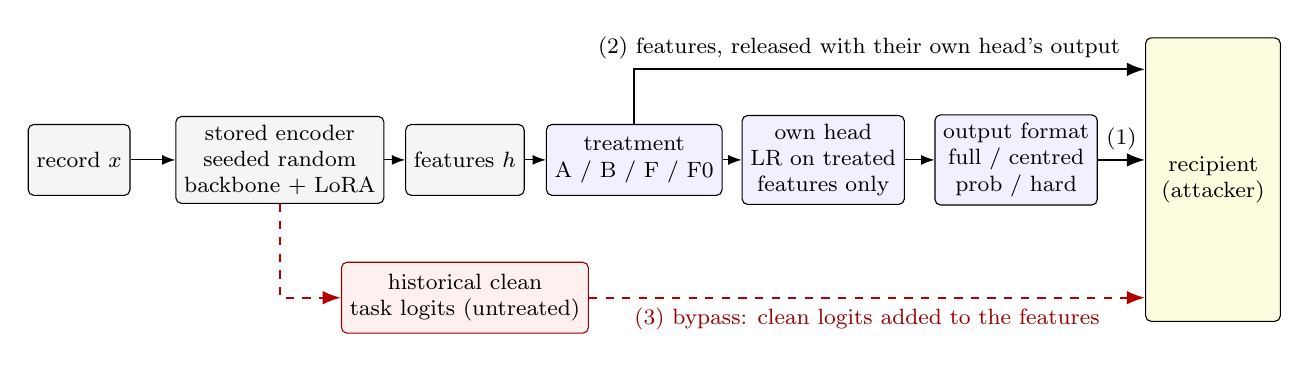
\begin{tikzpicture}[
  font=\footnotesize, >=Latex,
  box/.style={draw, rounded corners=2pt, align=center, minimum height=9mm, inner sep=3pt},
  own/.style={box, fill=black!4},
  rel/.style={box, fill=blue!6},
  bad/.style={box, fill=red!6, draw=red!60!black}]
  \node[own] (x) at (0,0) {record $x$};
  \node[own] (enc) at (2.55,0) {stored encoder\\seeded random\\backbone + LoRA};
  \node[own] (h) at (4.9,0) {features $h$};
  \node[rel] (arm) at (7.05,0) {treatment\\A / B / F / F0};
  \node[rel] (hd) at (9.45,0) {own head\\LR on treated\\features only};
  \node[rel] (out) at (11.9,0) {output format\\full / centred\\prob / hard};
  \node[box, fill=yellow!12, minimum height=36mm, text width=15mm] (rec) at (14.4,-0.25) {recipient\\(attacker)};
  \node[bad] (clean) at (4.9,-1.75) {historical clean\\task logits (untreated)};
  \draw[->] (x) -- (enc);
  \draw[->] (enc) -- (h);
  \draw[->] (h) -- (arm);
  \draw[->] (arm) -- (hd);
  \draw[->] (hd) -- (out);
  \draw[->, thick] (out) -- node[above]{(1)} (out -| rec.west);
  \draw[->, thick] (arm.north) |- node[pos=0.72, above]{(2) features, released with their own head's output} (rec.west |- 0,1.15);
  \draw[->, dashed, thick, red!70!black] (enc.south) |- (clean.west);
  \draw[->, dashed, thick, red!70!black] (clean.east) -- node[pos=0.5, below, text=red!60!black]{(3) bypass: clean logits added to the features} (clean -| rec.west);
\end{tikzpicture}
}
\caption{Recipient view. Solid paths are permitted releases: (1) output only, in one of four formats; (2) features of
a treatment (A untreated, B LEACE, F FARE, F0 zero-fairness FARE tree) released with the output of their own head,
which reads only those features. Path (1) is drawn for an own head (Experiment~4); in Experiments~1--3 the released
output is that of the frozen head, which reads the untreated features. The dashed path (3) adds the frozen head's clean
logits to the features; it is the bypass, evaluated only as an adverse control.}
\label{fig:recipient}
\end{figure}

\paragraph{Feature treatments.} A: the untreated representation. B: target LEACE~\citep{belrose2023leace}, in its
reference implementation (concept-erasure 0.2.4), which erases only the pair's protected attribute and is fitted on
\texttt{defense\_fit}. F: FARE~\citep{jovanovic2023fare}, in the authors' implementation, whose release is the one-hot
index of a tree cell. Its configuration comes from a frozen grid. Among the configurations whose probe accuracy on the
attacker's selection role is within one point of the untreated probe's, the one with the lowest validation recovery for
our nonlinear attacker is chosen. On HMDA the untreated task gain over the constant is only 0.6 to 2.3 points, so this
rule admits a constant release: on HMDA seed~1 the chosen configuration has a single cell, keeps none of the gain and
recovers 0.5 by construction, and on the other two HMDA seeds it has four cells. F0: the same FARE configuration with
fairness weight zero, that is, a tree of the same budget grown on the task label without the fairness term, so that it
only compresses. Experiment~1 also adds Gaussian noise to the representation, at the smallest scale $\sigma^*$ whose
validation recovery for our nonlinear attacker is at most 0.55 ($\sigma^*=2$ on Adult and 4 on HMDA). FARE and noise
were therefore tuned against the evaluated attacker slate on the attackers' own selection rows, which can favour them
when they are scored against the same slate; for noise, attackers outside the slate recovered more
(Section~\ref{sec:threat}). No defense grid was expanded and no configuration was re-selected after assessment.

\section{Threat model and access}\label{sec:threat}

\paragraph{The recipient and its release.} A \emph{recipient} is a party permitted one purpose. For each record it
serves, it receives that purpose's release under the contract in force and nothing else about the record: not the
record's inputs, its true task label or its protected attribute, and not the model's parameters, gradients or internal
states (defense maps, heads, or a representation that the contract does not release). Each record is released once, and
no recipient submits inputs of its choosing. For the noise treatment, noise is drawn once per record for each of three
release seeds; the three realizations are attacked separately and averaged, never pooled for one record. The label-only
reference of Section~\ref{sec:outputs} is a comparator, not a recipient: it reads the scored record's true task label.

\paragraph{Why this access.} The claims we evaluate concern a release policy, so we chose to evaluate an adversary that
holds what the policy delivers. That part of the access describes the service itself: an authorized recipient necessarily possesses the
information delivered to it. Two further capabilities are granted by the evaluation and are
not established for any deployment. The first is linkage. Two recipients that serve the same person may link their
releases by record, and the linked-recipient evaluation asks whether protection that holds for each recipient survives
when they pool. We grant perfect linkage, the attacker-favourable limit: a low pair recovery cannot be blamed on linkage
error, while a high one may overstate what a coalition with imperfect linkage would recover. We do not assume that
contracts or governance prevent linkage, and we do not claim that pooling is unavoidable. The second capability is
labelled auxiliary data: releases of other records from the same population together with their protected attribute.
This models a recipient that knows the attribute for some of the people it serves and can therefore learn how outputs
relate to the attribute, as in attribute-inference work in which attackers train on labelled examples or on people who
disclosed the attribute~\citep{song2020overlearning,jia2018attriguard}. The availability of such data, its size and its
match to the scored population are assumptions of the benchmark; we do not show that a recipient could obtain such data
in practice. Withholding the scored record's inputs isolates what the release itself reveals: with the inputs, recovery
could come from imputation rather than from the release~\citep{jayaraman2022imputation}. A recipient that holds inputs
is a separate threat model, not an illegitimate one. More access cannot lower what an optimal attacker recovers, so a
stronger attacker could recover more, but that alone does not justify granting more access. Each further capability,
such as a defense's fitted parameters, defines a separate threat model that needs its own justification. A stronger
attacker within the same access is different: a larger slate, or an attacker that uses public knowledge of a defense's
algorithm and objective while seeing only the releases, belongs to this threat model. Our slate is neither, so each
recovery figure is a lower estimate of what this access allows, not a guarantee.

\paragraph{Attackers.} Our attackers are supervised. Each is fitted on the releases of the records in the attacker's
fitting role, \texttt{attacker\_fit}, labelled with the protected attribute; it is chosen by log loss on the labelled
records of its selection role, \texttt{attacker\_val}; and it is scored on \texttt{assessment} records that no attacker
was fitted or selected on (Section~\ref{sec:protocol}). Tree and
neural attackers also hold out an internal 10\% of \texttt{attacker\_fit} for early stopping. The sizes of the two
labelled roles fix the attacker's data budget; they differ between experiments and are listed in
Table~\ref{tab:access}. The labelled sample is a requirement of these supervised attackers, not of every conceivable
attack, and attacks that need no labelled sample, for example ones built from a known population law, are not
evaluated. Attackers are refitted to the releases of the defended system and so adapt to the distribution that the
defense emits; only in that limited sense are they defense-aware. Knowing a defense's published algorithm and objective
is different from holding its fitted parameters. A recipient may know the former. The slate's attackers, whose recovery
the tables report, use neither beyond refitting to the defended releases; the one exception, run only in Experiment~1,
is described below. Records are assigned to roles by a hash of a canonical
record key, which also groups duplicate records; keys and row identifiers align releases and are never attacker
inputs.

\paragraph{What recovery measures.} Recovery is the held-out AUC that our attackers achieve. It describes a fixed
attacker slate under this threat model, so a better attacker might recover more, and it is not a privacy guarantee. A
difference in recovery between two treatments can reflect information about the attribute that one treatment removed,
limits of our attackers at this data budget, or both; our measurements do not separate the two. A low recovery
therefore does not show that the information is gone, and a high recovery does not show that all of it was kept. Being
deterministic or real-valued does not make a release reversible: a function of the representation can merge records,
and a deterministic map to probability vectors, which stays within a probability-output contract, can remove
information about the attribute. We do not establish whether any evaluated release keeps the population distribution of
the attribute given the record.

\paragraph{Access in each experiment.} Table~\ref{tab:access} gives, for each experiment, what the recipient receives,
the labelled sample, how the attackers are fitted, selected and scored, what they know about the defense, how releases
are linked, and what remains untested. The attackers of each experiment are described as they were implemented; no
experiment is credited with a capability that only a later evaluation added. Experiment~1 also ran two exploratory
attackers with more knowledge of the defense than the slate. On the noise treatment and the features-only surface only,
it fitted two closed-form Gaussian likelihood-ratio attackers that use the noise law, an isotropic Gaussian with the
selected scale $\sigma^*$, treated as a published parameter of the mechanism. The first is fitted, like the slate, on the
labelled noisy releases of \texttt{attacker\_fit}; it stays within the access above but uses knowledge of the defense's
algorithm and scale. The second is fitted on clean, pre-noise representations of the \texttt{attacker\_fit} records,
which no contract releases, and so exceeds the access above. Neither is an insider or repeated-query attack, and neither
has white-box access to the model: neither is selected on \texttt{attacker\_val}, both score one noisy release per
assessment record, and neither uses the encoder's or heads' parameters or gradients, or any assessment record's clean
representation. At $\sigma^*$ the first recovered 0.546 on Adult and 0.526 on HMDA, and the second 0.563 and 0.575, against 0.528
and 0.513 for the slate (exploratory values with unadjusted intervals and no paired test). The features-only noise entries
of Table~\ref{tab:summary} are therefore not the strongest attack that was run on that surface; no noise-aware attacker
was run on noisy features released with clean outputs.

\begin{table}[t]
\centering\footnotesize
\caption{Access in each experiment. Common to every attack of the slate: one release per record (noise: one draw per record for each
of three release seeds, attacked separately); attackers fitted on labelled \texttt{attacker\_fit} releases, selected by
\texttt{attacker\_val} log loss and scored on \texttt{assessment}; no attacker receives a record's inputs, model
parameters, gradients or defense maps, and record keys are never attacker inputs. The exploratory likelihood-ratio
attackers of Experiment~1 are the exception described in Section~\ref{sec:threat}: they use the noise scale, are not
selected, and one is fitted on clean auxiliary representations. Labelled sample: rows of
\texttt{attacker\_fit} / \texttt{attacker\_val}. The label-only reference reads the scored record's true task label and
is a comparator, not a recipient.}\label{tab:access}
\begin{tabular}{@{}L{2.2cm}L{4.6cm}L{2.5cm}L{5.6cm}@{}}
\toprule
Experiment & What the recipient receives & Labelled sample (Adult; HMDA) & Defense knowledge, linkage, untested access\\
\midrule
Encoders' stored check (a check, not an attack; reproduced in Exp.~1) & ridge fitted and scored in sample on the
64-dimensional representation of every test record & none; uses the scored records' own labels (15{,}060; 13{,}661) &
the method's own test; covers only linear prediction from the representation\\
\addlinespace
1. Feature removal (untreated and LEACE: all 14 pairs; noise: the two primary settings) & representation (untreated, LEACE,
or noise at $\sigma^*$ on the primary settings); representation with the untreated head's full logits; full logits only & 7{,}571 / 2{,}239; 6{,}794 / 2{,}089 & slate refitted to releases;
$\sigma^*$ chosen on \texttt{attacker\_val} with the slate; exploratory likelihood-ratio attackers know $\sigma$ (see
text). Features and output held by one recipient. Untested: repeated or fresh-noise queries, own-head outputs, other
formats, pairs, and noise on the secondary pairs (stopped by a budget rule; not reported)\\
\addlinespace
2. Finite releases and output formats & FARE or zero-fairness cell (one-hot) or representation; either with the
untreated head's full logits; frozen-head output as full logits, probabilities or hard decision; features with the
output of a head fitted on them, and that output alone (reused in Exp.~4); noisy features with each output format (not
reported) & 6{,}065 / 2{,}235;
5{,}388 / 2{,}082 (after removing 1{,}500 Adult and 1{,}385 HMDA rows for FARE certification) & slate refitted to releases; FARE configuration
chosen on \texttt{attacker\_val} with the slate; a cell-conditional attacker on some finite releases (descriptive). No
pairs. Untested: attacks using FARE's tree or objective, noise-aware attacks, repeated queries\\
\addlinespace
3. Output diagnosis & frozen-head output in six formats (full, centred, probabilities, offset, centred with offset,
hard) and two format banks (Section~\ref{sec:protocol}), and the same formats for a refitted logistic head on the primary settings; Adult income and
occupation-group outputs concatenated for one linked pair; features, own output or both on an easier task (Section~\ref{sec:compression}) & as Exp.~2
(pair and easier task: Adult only) & no defense on the frozen and pair outputs; FARE configuration on the easier task
chosen on \texttt{attacker\_val} with the slate, among configurations that also keep 80\% of the probe's gain; a
cell-conditional attacker on hard outputs and FARE cells (descriptive). Pair: perfect linkage granted by
aligned rows, linked labelled sample, single-recipient attackers among the candidates. Untested: imperfect linkage, more
than two recipients, pairs that include features or defended outputs, HMDA pairs\\
\addlinespace
4. Useful heads (Adult income / sex) & output of a logistic-regression head fitted on each treatment's features, in
four formats and two banks; features with own output; features only; features with the untreated head's logits & as
Exp.~2 (Adult) & slate refitted to releases; F is Exp.~2's configuration; a cell-conditional attacker on F and F0 outputs
and hard decisions (descriptive). No pairs. Untested: repeated queries, other head families, HMDA\\
\bottomrule
\end{tabular}
\end{table}

\paragraph{Threat models outside this evaluation.} The following are distinct threat models that we do not test.
Several involve no breach of the provider: a recipient may legitimately hold a person's inputs, a model may be
published, and a service may permit repeated queries. Some are governed by release-policy choices such as rate limits,
one release per person, query auditing and whether to publish the model; others need security controls. We claim no
protection against any of them and do not dismiss them: recipients that also hold a record's inputs or later learn its
true label; public or leaked model parameters or gradients; permitted repeated, adaptive or chosen-input queries,
including releases from several model versions; attacks that use a defense's fitted parameters, such as a LEACE map or
a FARE tree; insiders; imperfect linkage; coalitions of more than two recipients; and auxiliary samples larger or smaller
than ours, drawn from another population, or containing the auxiliary records' inputs or task labels. Within this
access, attackers that exploit a defense's published algorithm or objective were not run, apart from the exploratory
noise-aware attackers of Experiment~1, one of which also used the auxiliary records' pre-release representations.

\section{Related work}\label{sec:related}

\paragraph{Concept erasure and its evaluation.} Linear concept erasure aims to stop linear classifiers from recovering a
concept: INLP~\citep{ravfogel2020inlp} by iterative nullspace projection, R-LACE~\citep{ravfogel2022rlace} through a
linear minimax game, and LEACE~\citep{belrose2023leace}, which guarantees it in closed form, for the moments of the data it is fitted on,
with the least squared change among linear erasers. Such guarantees do not extend to nonlinear recipients: INLP and R-LACE report nonlinear recovery after
linear erasure, kernelized erasure does not transfer across kernels~\citep{ravfogel2022kernel}, and LEACE restricts its
claim to linear adversaries. Adversarially trained representations show the same pattern: post-hoc attackers recover
what the in-training adversary could not~\citep{elazar2018adversarial} and still read the attribute from adversarially
censored representations~\citep{song2020overlearning}, and independent post-hoc
adversaries are a standard check~\citep{moyer2018invariant}. Our LEACE measurements are a further instance.

\paragraph{Leakage through task outputs.} Model-inversion and attribute-inference attacks exploit confidence
scores~\citep{fredrikson2014pharmacogenetics,fredrikson2015model}; label-only attacks can match confidence-based
ones~\citep{mehnaz2022sensitive}, and masking confidences does not stop label-only membership
inference~\citep{choquettechoo2021label}. \citet{wang2019balanced} compare leakage from predictions with that implied
by the true labels at matched task performance; we report a label-only reference in the same spirit. A multiclass
log-linear head on a linearly guarded representation can still reveal the erased concept, although a binary one
cannot~\citep{ravfogel2023loglinear}. Black-box attribute inference on training records rarely
exceeds what an adversary with the same distributional knowledge achieves by imputation~\citep{jayaraman2022imputation},
so we report constant and label-only references. Coarsening outputs, for
example rounding confidences~\citep{fredrikson2015model}, is an old countermeasure; releasing probabilities rather than
logits leaves calibration~\citep{guo2017calibration} and every proper task loss unchanged.

\paragraph{Fair representations and trade-offs.} When the label depends on the protected attribute, fair
representations trade accuracy for protection~\citep{zhao2019inherent,zhao2022inherent}.
\citet{stadler2024lpl} prove that, for finite discrete data with full support and a strictly positive label posterior,
a representation that carries more information about the task label than a level $\gamma$ cannot keep, for
\emph{every} attribute, the inference gain of an adversary who sees it together with the label, over one who sees the
label alone, within that level. The violating attribute is constructed, and the authors note that leakage of a single
attribute can sometimes be restricted. We report an analogue of their label-only adversary as a descriptive comparison,
not a floor: in our setting the releases are computed from the inputs alone, so they can reveal less, or more, than the
true label does. In Experiment~2 the frozen heads' full outputs revealed more than the label-only reference and their
hard decisions revealed less (exploratory). Adversarial methods such as LAFTR~\citep{madras2018laftr} lack guarantees against unseen
classifiers; FCRL~\citep{gupta2021fcrl} evaluates with a common downstream protocol. FARE~\citep{jovanovic2023fare}
restricts the encoder to a finite partition and certifies, with probability at least $1-\epsilon$, a bound on the
demographic-parity distance of any classifier that reads only the cell; its authors note that restricted encoders lose information and compare fairness-unaware $k$-means
encoders. We add a same-budget zero-fairness tree and measure attribute recovery from the complete release.

\paragraph{Adversary models and combined releases.} Our recipient is not a new adversary. It is the auxiliary-data
attacker of attribute inference, which learns from labelled examples to read a sensitive attribute from what a model
exposes~\citep{song2020overlearning} or from a person's public data~\citep{jia2018attriguard}, applied here to released
task outputs as well as representations. Combining independent releases is a classical route to breaches~\citep{ganta2008composition}; recipients
of differently perturbed copies of the same data can pool them, and mechanisms exist under which the pool reconstructs
the data, by linear least-squares estimation, no more accurately than the best single copy~\citep{li2012multilevel}; an
attack that combines the predictions of a biased and a fair version of one model raises attribute inference on image
benchmarks~\citep{tian2025fairnessprivacy}; and collusion-aware mechanisms exist
for sequential finite-alphabet releases~\citep{taylor2026collusion}. We measure the case in which each recipient is permitted a different purpose, as a property of our attackers.

\paragraph{Position.} In our reading of the closest work on concept erasure, fair representations, output leakage
and combined releases, we did not find one protocol that applies, on the same
stored models, each method's native check, nonlinear recovery from representation and complete output, the released
output's held-out utility, a capacity-matched zero-fairness control, and recipient pairs. FARE is closest on matched
utility and compression, \citet{wang2019balanced} on utility-qualified output leakage, and
\citet{tian2025fairnessprivacy} on combined releases. This reflects a bounded search and is not a claim of priority.

\section{Evaluation protocol}\label{sec:protocol}

\paragraph{Experiments.} The evidence comes from four experiments on the same stored models. They share the attacker
slate and the endpoint discipline described below, but they were run separately, with their own registered endpoints,
and they differ in roles (Table~\ref{tab:access} gives each experiment's labelled budget) and in how intervals are
computed. Experiment~1 compares untreated and LEACE representations on all 14 pairs, and noisy representations at
$\sigma^*$ on the two primary settings. Experiment~2 adds official FARE and the zero-fairness tree, and compares the frozen
heads' full logits with their hard decisions. Experiment~3 measures the effect of withholding the logit offset, the
usefulness of the frozen heads, a two-recipient pair, and FARE's compression share on an easier task. Experiment~4
replaces the frozen heads with a useful head fitted on each treatment's features. Table~\ref{tab:access} gives each
experiment's access.

\paragraph{Roles.} Experiments~2--4 use the same record-group roles: \texttt{defense\_fit} (owner side: the encoders' own
training split of 24{,}127 Adult and 63{,}704 HMDA records, on which LEACE maps, FARE trees and task heads are fitted,
with a 20\% head holdout for head selection), \texttt{attacker\_fit} and \texttt{attacker\_val}
(attacker fitting and selection), and \texttt{assessment} (scoring only: 5{,}243 Adult and 4{,}764 HMDA records).
Records that also occur in the encoder's training split are excluded from every scored role (17 Adult and 42 HMDA test
records), and a further 20\% of \texttt{attacker\_fit} groups is reserved for FARE certification. The owner also uses
the attacker roles: the task labels of \texttt{attacker\_fit} fit the common utility probe and those of
\texttt{attacker\_val} select it and decide which FARE configurations are admissible, while the protected labels of
\texttt{attacker\_val} choose FARE's configuration and, in Experiment~1's roles, the noise scale
(Section~\ref{sec:setting}). No sensitive
assessment label selects a release, grouping, penalty, attacker or utility probe. Experiment~1 used the original roles (assessment 5{,}250 Adult and 4{,}778 HMDA records), which retained
the overlapping records; its verdicts were stable when they were removed.

\paragraph{Attackers and recovery.} Every reported surface is attacked by the same slate, with the access of
Section~\ref{sec:threat}: logistic regression (5 regularisation values), gradient-boosted trees (20 configurations) and
an MLP (18), each fitted on \texttt{attacker\_fit} releases labelled with the protected attribute. The nonlinear
attacker is the better of the tree and MLP families on \texttt{attacker\_val} log loss, refitted at three attacker
seeds. Recovery is the nonlinear attacker's macro one-vs-rest AUC on assessment over supported classes
(Section~\ref{sec:setting}), averaged over attacker seeds, release
realizations (noise only) and then encoder seeds. For releases that combine features and output, selection on validation also considers attackers
that use only the features or only the output. For the recipient pair of Experiment~3, the candidates also include each single recipient's
attacker, chosen on validation like any other candidate. For some finite releases (Table~\ref{tab:access}) we
additionally fit a cell-conditional attacker, which estimates the attribute's distribution within each released cell;
we report it descriptively, and where both were fitted it matched the nonlinear attacker. In Experiments~3 and~4 a
\emph{bank} is a set of release formats of the same output; for each encoder seed the format whose nonlinear attacker
has the lowest validation log loss is scored. The full bank includes the full logits and the offset-free bank does not.
The label-only and constant references, the cell-conditional attacker, the exploratory likelihood-ratio attackers of
Section~\ref{sec:threat} and the encoders' in-sample check are not part of the slate.

\paragraph{Utility.} In Experiments~3 and~4 we report the accuracy, balanced accuracy, minority recall, log loss and gain
over the constant (majority class on \texttt{attacker\_fit}) of the \emph{deployed} head whose output is released.
Experiments~1 and~2 report the accuracy of a common refitted probe, and Experiment~2 also the accuracy and log loss of
the head fitted on each treatment's features.

\paragraph{Native checks.} The encoders' stored check is a historical value, the in-sample one-hot ridge $R^2$ on the
test split with threshold 0.05, which Experiment~1 reproduced on all 42 combinations of pair and encoder seed. LEACE's
implementation bound is a whitened residual cross-covariance below its tolerance on \texttt{defense\_fit}. FARE's is
its demographic-parity certificate ($\epsilon=0.05$) on the certification role (1{,}500 Adult and 1{,}385 HMDA rows).

\paragraph{Inference.} Each endpoint is a mean over encoder seeds of a per-seed statistic. In Experiments~3 and~4,
standard errors come from 1{,}999 paired multinomial bootstrap replicates over assessment record groups, shared by every
attacker fit, and intervals are simultaneous two-sided 95\% Bonferroni normal intervals over the endpoint family. All intervals
describe the mean over the three stored encoders, conditional on the fitted heads and attackers; they do not cover the
variation from retraining encoders, which is large (Figure~\ref{fig:useful}).
Experiments~1 and~2 used one-sided Bonferroni percentile bounds from 20{,}000 group-bootstrap replicates
over endpoint families of 24 and 12 ($\alpha=0.05/24$ and $0.05/12$), and the bounds
in Table~\ref{tab:summary} from those experiments are of that kind. In every experiment an endpoint passes only if its
lower bound exceeds its registered target. Utility targets are a non-inferiority margin of $-0.01$, a gain of $0.03$,
and the retention contrast $\Acc(\text{treatment})-0.8\,\Acc(A)-0.2\,\Acc(\text{const})>0$, which requires a treatment to
keep at least 80\% of the untreated head's accuracy gain over the constant; the recovery contrasts of Experiments~2--4 use a target of $0.02$ AUC.
Experiment~1's registered endpoints compare levels with fixed bars instead (recovery with 0.55 AUC, the held-out linear
statistic with 0.05 and probe accuracy with a one-point margin), and Experiment~3's frozen-head usefulness endpoints
used a gain target of 0.01. An interval that excludes zero but not the
target is reported as a smaller difference below the target, never as ``no difference''; an endpoint is \emph{not established} when its lower bound does not exceed the target,
which is not evidence of no effect. Each experiment was \emph{registered}: its protocol, code, input hashes, list of fits and endpoint families were
committed to the anonymous repository, with timestamps, before its first fit, and an independent replay that
does not import the analysis code recomputed every primary result. The encoders' stored check predates these
experiments; Experiment~1 reproduced its values. Three changes were made after runs had begun, and each is recorded with
its protocol: a guard in Experiment~2's FARE certification code that identifies duplicate rows by record rather than by
feature values, without which every certificate was unavailable; a scoring repair to the easier-task comparison of
Experiment~3, found by the independent replay, which applied the registered rule for candidates that ignore one part and
moved that endpoint's lower bound from 0.0001 to 0.0019 without changing its verdict; and reporting repairs in
Experiment~3 that changed no estimand, selection, role or verdict.

\section{Results}\label{sec:results}

Table~\ref{tab:summary} collects the main contrasts from Experiments~1--3. Section~\ref{sec:useful} reports the
useful-head comparison, and Sections~\ref{sec:compression} and~\ref{sec:pairs} the compression share of FARE's effect
and the linked recipients.

\begin{table}[t]
\centering\small
\caption{Main contrasts from Experiments~1--3 (means over three encoder seeds; the noise row also averages three
release seeds). Parenthesised values are lower confidence bounds of registered contrasts: a one-sided Bonferroni
percentile bound in Experiment~2 and lower ends of simultaneous two-sided Bonferroni intervals in Experiment~3
(Section~\ref{sec:protocol}). Several other rows are registered levels or contrasts whose bounds are reported with the
experiments.}\label{tab:summary}
\begin{tabular}{@{}L{5.5cm}ccc@{}}
\toprule
Quantity & Exp. & Adult income / sex & HMDA underwriting / race\\
\midrule
Encoders' own linear check fails (pair$\times$seed, all 14 pairs) & 1 & \multicolumn{2}{c}{11 of 42}\\
Nonlinear recovery, untreated features & 1 & 0.815 & 0.870\\
Nonlinear recovery, LEACE features & 1 & 0.817 & 0.863\\
Noise at $\sigma^*$, features only / plus clean outputs & 1 & 0.528 / 0.778 & 0.513 / 0.758\\
Full logits vs hard decision (frozen head) & 2 & 0.776 vs 0.513: +0.263 (0.249) & 0.768 vs 0.505: +0.262 (0.254)\\
FARE vs LEACE features & 2 & 0.550 vs 0.812 & 0.501 vs 0.863\\
Zero-fairness tree (same budget), features & 2 & 0.645 & 0.608\\
FARE features plus historical clean outputs & 2 & 0.788 & 0.768\\
Offset withheld: full bank minus offset-free bank & 3 & +0.072 (0.062) & +0.067 (0.060)\\
\quad per encoder seed & 3 & 0.079 / 0.064 / 0.072 & 0.058 / $-$0.0003 / 0.143\\
Frozen head: accuracy gain over constant (target 0.01) & 3 & 0.039 (0.031) & 0.016 (0.0098), not established\\
\bottomrule
\end{tabular}
\end{table}

\subsection{What each method's own check establishes}\label{sec:native}

Three outcomes have to be kept apart: a method failing its own test, its test holding while recovery occurs outside the
test's scope, and recovery through a surface that the test does not cover. The encoders' constraint is an instance of
the first. Their stored linear check fails on 11 of the 42 untreated combinations (14 purpose--attribute pairs, three encoder
seeds each), including HMDA
underwriting/race on two of three seeds, so for those combinations the encoders do not deliver the protection that their
own test describes. LEACE is an instance of the second. It meets its bound on all 60 fitted maps (including 18 fitted for a set of
attributes), and its held-out squared top canonical correlation $\rho_1^2$ is small (point estimates 0.0006 on Adult
and 0.0001 on HMDA, with unadjusted 90\% upper ends of 0.013 and 0.033, on one already-used held-out split). This is a
measurement on one split, not a guarantee about future records, and on seeds whose \texttt{defense\_fit} covariance is
rank-deficient LEACE leaves directions outside its fitting support unchanged. Nonlinear recovery nevertheless changes by less than 0.01 AUC (Adult $+0.002$, HMDA $-0.007$, from the levels in Table~\ref{tab:summary}; for HMDA the unadjusted 90\% interval of the
change excludes zero). The guarantee concerns linear
classifiers, and this measurement shows that our nonlinear attackers still recover the attribute about as well as from
untreated features; it is not evidence against the theorem. FARE's certificate could not be assessed in the same way. At the available certification sizes it was unavailable (the procedure could not run, for example
because a cell was absent from one certification split), vacuous (a bound above 1) or weak (Adult bounds about 0.50), and its only informative bound (0.175, a secondary certificate over three race groups) belongs to a degenerate HMDA
configuration with a single cell. These certificates exist only after the post-run repair of the certification code
described in Section~\ref{sec:protocol}.

\subsection{The task output as a separate surface}\label{sec:outputs}

The third outcome concerns what a feature defense does not cover. Output-only recovery exceeds the label-only reference
by 0.177 on Adult and 0.236 on HMDA, so the outputs carry information about the attribute beyond what the true label
carries. When the clean output is released beside noisy or FARE features, recovery returns to 0.76--0.79
(Table~\ref{tab:summary}). This is expected, because the clean output alone already recovers 0.776 on Adult and 0.768 on
HMDA. The defenses make no claim about outputs; the measurement shows that a feature defense cannot be credited with
protection when the original output is sent with the features.

\subsection{Withholding the logit offset}\label{sec:offset}

The common logit offset changes no probability, decision or task loss, yet the frozen heads release it as part of their
full logits. Withholding it lowered recovery by 0.072 (Adult) and 0.067 (HMDA) AUC. The effect appeared on 5 of the 6
primary encoder seeds and was absent on the collapsed HMDA seed~1. Across the 14 stored pairs it was established on 5.
It was not established for any of the six multiclass Adult pairs, but it passed for the five-class HMDA pricing head with
race. For a refitted logistic-regression head whose logits are log-probabilities, the offset is a function of the
margin, so the effect is zero by construction; that head is about twice as useful (gain 0.083), and its margin alone
recovers 0.773. The result is therefore a measurement of an output contract for particular frozen heads, and it does not
amount to a general method: it depends on how the heads were trained and disappears for heads whose logits carry no
free offset. It is relevant wherever a service returns raw logits.

\subsection{Low decision-level recovery and usefulness}\label{sec:frozen}

The frozen heads' hard decisions leak little (0.513 on Adult, 0.505 on HMDA), but those decisions are weakly useful. The
Adult frozen head gains 3--5 accuracy points over a constant and recalls 14--22\% of high earners. HMDA underwriting
usefulness is not established (lower bound 0.0098 against a target of 0.01). The HMDA fair-lending head predicts the
same class for everyone, although its scores still vary and are informative about race and sex (centred-logit recovery
0.646 and 0.655). Low decision-level recovery here coincides with decisions that barely beat a constant. This matters
for any reading of hard decisions as a defense: on these heads the low recovery cannot be separated from the low
usefulness, which is why Experiment~4 repeats the comparison with useful heads.

\subsection{Matched useful-head comparison}\label{sec:useful}

\paragraph{Design.} On Adult income/sex, every treatment releases the output of a logistic-regression head from one
common family (regularisation grid fitted on \texttt{defense\_fit} minus a holdout, selected on holdout log loss) whose
only runtime input is that treatment's features. The heads, LEACE maps and FARE trees are reused unchanged, and so, after checking their hashes, are four
surfaces from Experiment~2: full logits alone, features alone, features with full logits, and the bypass. Experiment~2
had already reported their levels in exploratory tables. The centred, probability and hard surfaces and
the banks are new and were fitted after the protocol was registered (3{,}924 model fits). Because the heads emit
log-probabilities, their full logits, centred margin and probabilities are functions of one another and carry the same
information (verified to $10^{-12}$). The ten primary recovery endpoints use the centred and hard formats; the other
nine primary endpoints concern utility.

\begin{figure}[t]
\centering
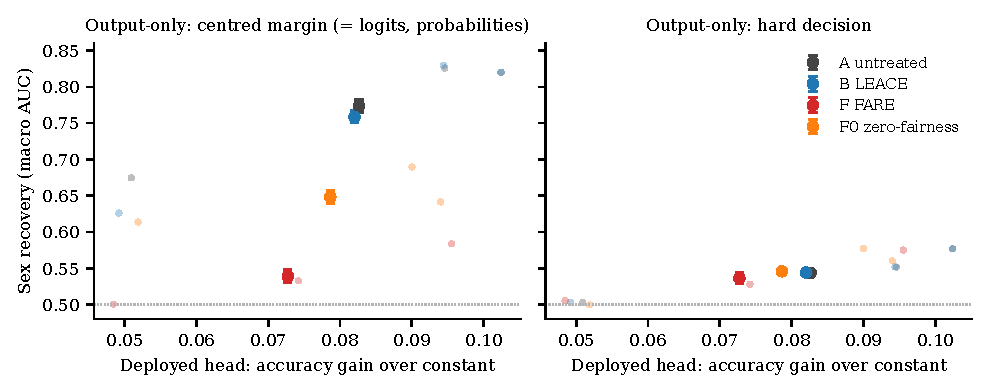
\includegraphics[width=\linewidth]{figures/fig_useful_head.pdf}
\caption{Useful-head comparison on Adult income/sex. Each treatment releases the output of a deployable
logistic-regression head fitted on its own features. Left: the centred margin, which carries the same information as the
head's logits and probabilities; right: the hard decision. Horizontal axis: the deployed head's accuracy gain over the
constant; vertical axis: sex recovery (macro AUC). Large markers: means over three encoder seeds with marginal 90\%
intervals (the simultaneous intervals of the registered endpoints are in Table~\ref{tab:useful}); small pale markers: individual seeds. The dotted line is chance.}\label{fig:useful}
\end{figure}

\begin{table}[t]
\centering\small
\caption{Primary useful-head endpoints (19; Bonferroni $z=3.008$). $\Acc$ is the deployed head's accuracy and $\Rec$
the nonlinear attacker's output-only recovery; every recovery row has the target $0.02$. Intervals are simultaneous
two-sided 95\% Bonferroni normal intervals; for gain and retention only their lower ends are shown. n.e.: not
established; ``excl.\ 0'': the lower bound is above zero but not above the target (here the whole interval lies below
0.02).}\label{tab:useful}
\begin{tabular}{@{}lccl@{}}
\toprule
Endpoint (target) & Point & Interval & Verdict\\
\midrule
$\Acc(B)-\Acc(A)$ ($>-0.01$) & $-0.0006$ & [$-0.0016$, 0.0003] & pass\\
$\Acc(F)-\Acc(A)$ ($>-0.01$) & $-0.0099$ & [$-0.0152$, $-0.0046$] & n.e.\\
$\Acc(\mathrm{F0})-\Acc(A)$ ($>-0.01$) & $-0.0040$ & [$-0.0086$, 0.0005] & pass\\
Gain over constant, B / F / F0 ($>0.03$) & 0.082 / 0.073 / 0.079 & $\ge$0.067 / 0.057 / 0.063 & pass\\
Retention, B / F / F0 ($>0$) & 0.016 / 0.007 / 0.013 & $\ge$0.013 / 0.001 / 0.007 & pass\\
\midrule
Centred: $\Rec(A)-\Rec(B)$ ($>0.02$) & 0.015 & [0.011, 0.019] & n.e.\ (excl.\ 0)\\
Centred: $\Rec(A)-\Rec(F)$ & 0.234 & [0.217, 0.252] & pass\\
Centred: $\Rec(A)-\Rec(\mathrm{F0})$ & 0.125 & [0.112, 0.139] & pass\\
Centred: $\Rec(B)-\Rec(F)$ & 0.220 & [0.201, 0.238] & pass\\
Centred: $\Rec(\mathrm{F0})-\Rec(F)$ & 0.109 & [0.092, 0.126] & pass\\
Hard: all five contrasts & $-0.002$ to 0.010 & lower bounds $<0$ & n.e.\\
\bottomrule
\end{tabular}
\end{table}

\paragraph{Utility.} All four heads are useful (Figure~\ref{fig:useful}, Table~\ref{tab:useful}): accuracy 0.832 (A),
0.831 (B), 0.822 (F) and 0.828 (F0) against a constant of 0.749, with balanced accuracy 0.72--0.73 and about half of high
earners recalled. LEACE and the zero-fairness tree are non-inferior within one point. FARE is not established as
non-inferior (lower bound $-0.015$), because seed~2 loses 2.0 points; it passes the gain and retention criteria, the
latter narrowly.

\paragraph{Recovery from useful scores.} The untreated head's score recovers sex at 0.773 and the LEACE head's at 0.759,
a smaller difference of 0.015 that lies below the registered target and is carried by seed~0 alone. FARE's head
recovers 0.539 and the zero-fairness tree's 0.648. Of FARE's 0.234 reduction, compression accounts for 0.125 and the
fairness term for a further 0.109, and the fairness-term contrast is positive on each seed. Post hoc and descriptively, a linear attacker on the untreated head's
margin recovers only 0.515, while nonlinear attackers on the same scalar recover 0.773. This is consistent with, but does
not establish, the reading that the sex signal left in the score is not linearly decodable and so lies outside a linear
eraser's scope.

\paragraph{Recovery from useful decisions.} When only the decision is released, every treatment recovers 0.536--0.546
and no contrast is established. The decision has the same accuracy as the score it comes from. Post hoc and
descriptively, the untreated head's decisions leak about as much as FARE's scores (difference $+0.005$, 90\% interval
[$-0.003$, 0.013]) while being about one point more accurate.

\paragraph{Complete release.} With features plus own output, recovery is close to that of the features alone (A 0.816, B 0.817,
F 0.550, F0 0.646), as expected, because the own head reads only those features. No offset effect was established for these heads, and none is possible in information terms, because their
offset is a function of the margin. Adding the clean output to F or F0 features brings recovery back to 0.788 and 0.789.

\paragraph{Registered predictions.} Four of the ten primary recovery predictions were correct: the contrasts of the
untreated score with FARE's and with the zero-fairness tree's, and the two hard-decision contrasts that we predicted
would not be established. The six wrong predictions were a larger LEACE effect on the score, a smaller fairness-term
effect on the score (we predicted that $\Rec(B)-\Rec(F)$ and $\Rec(\mathrm{F0})-\Rec(F)$ would not be established, and
both passed), and three established hard-decision contrasts against the untreated head. The predictions were
registered after full-logit recovery of these same heads had been reported as exploratory in Experiment~2, and the
protocol did not disclose that; we disclose it here.

\subsection{How much of FARE's effect is compression?}\label{sec:compression}

The answer differs between settings. On Adult income/sex, the zero-fairness tree's features recover 0.645 against FARE's 0.550
and LEACE's 0.812 (Experiment~2). The fairness term removes 0.109 beyond compression from the head's score
(Section~\ref{sec:useful}) and 0.096 [0.076, 0.116] from the complete release of features with the head's output (a
secondary endpoint of Experiment~4). On an easier task chosen by a screen that used only validation data (Adult occupation group with
age group protected; probe accuracy 0.974 for FARE and 0.975 untreated, against a constant of 0.277), FARE's
complete-release recovery is 0.151 below LEACE's, but the zero-fairness tree reproduces most of that reduction: on the
same complete-release surface, FARE's additional improvement is a smaller difference of 0.0074 [0.0019, 0.0129], below
the registered 0.02 target. That task is easy, but it is not a recoding of a single input column, which would make the
comparison trivial. An effect attributed to a fairness term therefore has to be measured against a capacity-matched
tree.

\subsection{Linked recipients}\label{sec:pairs}

\begin{figure}[t]
\centering
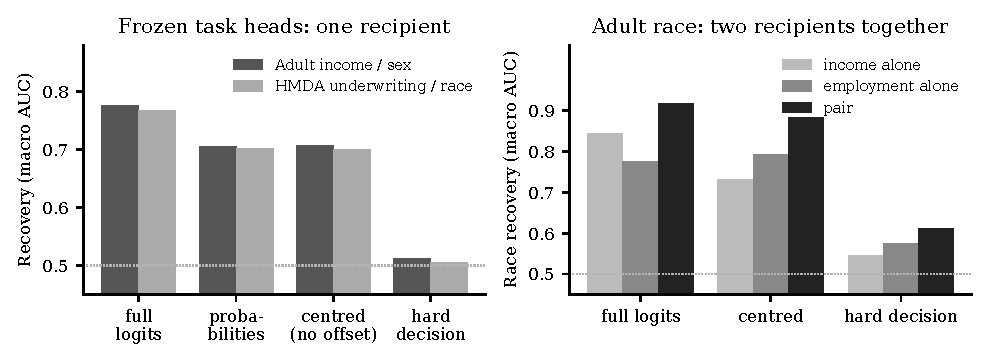
\includegraphics[width=\linewidth]{figures/fig_formats_pairs.pdf}
\caption{Left: recovery from the frozen heads' outputs by release format (Adult income/sex, HMDA underwriting/race).
Right: race recovery on Adult from the income recipient, the occupation-group recipient (labelled ``employment'') and
both linked, by format. Bars are means over three encoder seeds and show no intervals; the vertical axes start
near 0.45.}
\label{fig:pairs}
\end{figure}

We evaluated one coalition: two Adult recipients, each permitted only its own task output (income; occupation group)
from the untreated frozen heads, whose outputs are linked by record and pooled to recover race (macro AUC over the three Adult race
groups with enough records; the other two are not estimable), which is disallowed for both (Figure~\ref{fig:pairs}). The linkage is granted by aligning rows, and no linkage procedure is evaluated. In this family of
registered secondary endpoints, the pair beats both single recipients by more than 0.02 AUC under every format: full logits 0.917 against 0.845, centred 0.883 against 0.792, and
hard decisions 0.611 against 0.576 (pair minus the better single recipient $+0.034$, lower bound 0.023; this is the weakest of the six registered
contrasts of the pair against each single recipient under each format, all of which pass). We
report absolute pair recovery and its increment over the strongest single release separately. On seed~2 under full
logits, validation selected the income-only attacker for the pair, so that seed's pair-minus-income difference is exactly zero, which makes the pair estimate conservative
for that seed. Under the full and centred contracts each single-recipient comparator chooses among formats, while the
pair attacker sees only the contract's format, so the comparison, if anything, understates the pair's increment. These
are measurements with a fixed attacker slate under perfect linkage. They show that linked outputs
need an evaluation of their own; they do not show that race is carried only jointly by the two outputs. AUC is not an information measure. The pair gain does not separate evidence that each output carries on its own from
evidence present only in their combination, and we prove no composition or synergy result.

\section{Discussion}\label{sec:discussion}

\paragraph{Where the remaining recovery comes from.} LEACE's promise held wherever we could check it, FARE's
certificate was too weak at our certification sizes to be checked, and the encoders' own linear constraint failed its
check on 11 of 42 combinations. Apart from that failure, the recovery that remained came from attacker classes or
surfaces that the promises do not cover: nonlinear attackers on LEACE features, task outputs released beside defended
features, and a second recipient whose outputs are linked to the first. This is why the three outcomes of
Section~\ref{sec:native} are reported separately. A method can meet its own promise while the release as a whole
remains informative about the attribute.

\paragraph{What lowered recovery at matched utility, and what limits that reading.} Among the treatments that kept the
deployed head's accuracy within one point, LEACE barely changed what the score reveals and the zero-fairness tree
lowered it to 0.648. FARE lowered it further, to 0.539, and its fairness-term contrast was positive on each seed. Three
results limit what this supports. FARE's accuracy is not shown to be within one point of the untreated head, so its
larger reduction is not established at matched utility. On an easier task the same-budget tree reproduced most of
FARE's effect. And every feature defense that we evaluated together with the clean output was bypassed by it.
Releasing only the decision kept accuracy and gave the lowest recovery for every treatment, at the cost of discarding
scores that a recipient may need; with useful heads, decisions still recovered only 0.536--0.546, so their low recovery
is not explained by weak usefulness alone.

\paragraph{A measured gap (post hoc, descriptive).} At matched accuracy (within one point, established), the lowest
score-level recovery among the evaluated treatments is the zero-fairness tree's 0.648, while the untreated decision,
which has the same accuracy and no scores, recovers 0.544. Because a decision is a function of its score, this gap of
about 0.10 AUC measures how much more the scores reveal about the attribute than their thresholded decisions do, in this
setting. A method that released calibrated, useful scores with recovery near the decision's level would close it. We do
not claim that such a method exists, nor that it is impossible.

\paragraph{What the findings ask of future methods.} A method that aims to limit what recipients learn should state the
surfaces it covers and the access model under which it is evaluated, including the attacker's labelled-data budget, and
it should report recovery on the complete release beside the utility of the released output. An effect attributed to a
fairness term should be measured against a capacity-matched control, and a service whose recipients share people should
also be evaluated on linked releases. These are requirements for evaluating a method; they do not show that any
particular method fails them.

\section{Limitations, reproducibility, ethics and LLM assistance}\label{sec:limits}

\paragraph{Limitations.} The evidence covers two datasets, a small number of primary settings and three encoder seeds,
and the encoder seeds differ strongly (the HMDA encoder with seed~1 is collapsed). All assessment rows were used
before, so nothing here is fresh confirmation. Intervals are conditional on fitted heads and attackers and omit the
variation from retraining encoders. FARE is applied to stored representations rather than raw inputs, so its trees
partition the encoders' representations. The two smallest HMDA race groups have too few records to enter the macro AUC.
FARE's configuration and the noise scale were selected with the same attacker slate that scores them. The threat model
of Section~\ref{sec:threat} is one of several, and the threat models listed there are untested.
Several observations in Section~\ref{sec:useful} are post hoc and labelled as such.

\paragraph{Reproducibility.} For every experiment the protocol, code version, input hashes, list of fits and endpoint
families were committed before fitting. Result tables, inference code and the independent replay are in the
anonymous repository; per-record outputs, weights and checkpoints are kept privately with hash indexes. The encoders' public code still exposes an earlier bound from linear $R^2$ to classifier
accuracy that was later shown not to hold; we do not use it. The useful-head
comparison used about 0.25 CPU-hours on a laptop.

\paragraph{Ethics.} We study recovery of declared protected attributes from public benchmark data to inform release
policies. Attack code is standard; we release no per-person predictions.

\paragraph{LLM assistance.} A large language model assisted with code, analysis scripts, independent-replay scripts,
literature checking and drafting. All numbers were produced by committed code. A replay that does not import the analysis code
recomputed every registered endpoint; the post hoc diagnostics, the per-seed offset values and the refitted head's gain
(each recomputed separately) and the intervals drawn in Figure~\ref{fig:useful} were not part of that replay. The
authors are responsible for the content.

\bibliographystyle{plainnat}
\bibliography{references}

\end{document}
